% Options for packages loaded elsewhere
\PassOptionsToPackage{unicode}{hyperref}
\PassOptionsToPackage{hyphens}{url}
%
\documentclass[
]{article}
\usepackage{amsmath,amssymb}
\usepackage{lmodern}
\usepackage{iftex}
\ifPDFTeX
  \usepackage[T1]{fontenc}
  \usepackage[utf8]{inputenc}
  \usepackage{textcomp} % provide euro and other symbols
\else % if luatex or xetex
  \ifXeTeX
    \usepackage{zxjatype} 
    \usepackage[ipaex]{zxjafont}
  \fi
  \usepackage{unicode-math}
  \defaultfontfeatures{Scale=MatchLowercase}
  \defaultfontfeatures[\rmfamily]{Ligatures=TeX,Scale=1}
\fi
% Use upquote if available, for straight quotes in verbatim environments
\IfFileExists{upquote.sty}{\usepackage{upquote}}{}
\IfFileExists{microtype.sty}{% use microtype if available
  \usepackage[]{microtype}
  \UseMicrotypeSet[protrusion]{basicmath} % disable protrusion for tt fonts
}{}
\makeatletter
\@ifundefined{KOMAClassName}{% if non-KOMA class
  \IfFileExists{parskip.sty}{%
    \usepackage{parskip}
  }{% else
    \setlength{\parindent}{0pt}
    \setlength{\parskip}{6pt plus 2pt minus 1pt}}
}{% if KOMA class
  \KOMAoptions{parskip=half}}
\makeatother
\usepackage{xcolor}
\IfFileExists{xurl.sty}{\usepackage{xurl}}{} % add URL line breaks if available
\IfFileExists{bookmark.sty}{\usepackage{bookmark}}{\usepackage{hyperref}}
\hypersetup{
  pdftitle={Charitable Giving, Tax Reform, and Self-selection of Tax Report: Evidence from South Korea},
  hidelinks,
  pdfcreator={LaTeX via pandoc}}
\urlstyle{same} % disable monospaced font for URLs
\usepackage{longtable,booktabs,array}
\usepackage{threeparttable, threeparttablex, multirow}
\usepackage{calc} % for calculating minipage widths
% Correct order of tables after \paragraph or \subparagraph
\usepackage{etoolbox}
\makeatletter
\patchcmd\longtable{\par}{\if@noskipsec\mbox{}\fi\par}{}{}
\makeatother
% Allow footnotes in longtable head/foot
\IfFileExists{footnotehyper.sty}{\usepackage{footnotehyper}}{\usepackage{footnote}}
\makesavenoteenv{longtable}
\usepackage{graphicx}
\makeatletter
\def\maxwidth{\ifdim\Gin@nat@width>\linewidth\linewidth\else\Gin@nat@width\fi}
\def\maxheight{\ifdim\Gin@nat@height>\textheight\textheight\else\Gin@nat@height\fi}
\makeatother
% Scale images if necessary, so that they will not overflow the page
% margins by default, and it is still possible to overwrite the defaults
% using explicit options in \includegraphics[width, height, ...]{}
\setkeys{Gin}{width=\maxwidth,height=\maxheight,keepaspectratio}
% Set default figure placement to htbp
\makeatletter
\def\fps@figure{htbp}
\makeatother
\setlength{\emergencystretch}{3em} % prevent overfull lines
\providecommand{\tightlist}{%
  \setlength{\itemsep}{0pt}\setlength{\parskip}{0pt}}
\setcounter{secnumdepth}{5}
\newlength{\cslhangindent}
\setlength{\cslhangindent}{1.5em}
\newlength{\csllabelwidth}
\setlength{\csllabelwidth}{3em}
\newlength{\cslentryspacingunit} % times entry-spacing
\setlength{\cslentryspacingunit}{\parskip}
\newenvironment{CSLReferences}[2] % #1 hanging-ident, #2 entry spacing
 {% don't indent paragraphs
  \setlength{\parindent}{0pt}
  % turn on hanging indent if param 1 is 1
  \ifodd #1
  \let\oldpar\par
  \def\par{\hangindent=\cslhangindent\oldpar}
  \fi
  % set entry spacing
  \setlength{\parskip}{#2\cslentryspacingunit}
 }%
 {}
\usepackage{calc}
\newcommand{\CSLBlock}[1]{#1\hfill\break}
\newcommand{\CSLLeftMargin}[1]{\parbox[t]{\csllabelwidth}{#1}}
\newcommand{\CSLRightInline}[1]{\parbox[t]{\linewidth - \csllabelwidth}{#1}\break}
\newcommand{\CSLIndent}[1]{\hspace{\cslhangindent}#1}
\ifLuaTeX
  \usepackage{selnolig}  % disable illegal ligatures
\fi

\title{Charitable Giving, Tax Reform, and Self-selection of Tax Report: Evidence from South Korea}


      \usepackage{authblk}
                            \author[]{Hiroki Kato}
                                      \affil{Osaka University}
                                                    \author[]{Tsuyoshi Goto}
                                      \affil{Chiba University}
                                                    \author[]{Yong-Rok Kim}
                                      \affil{Kobe University}
                              
\date{2021/07/21}


\begin{document}
\maketitle
\begin{abstract}
This paper investigates (1) the price elasticity of giving and (2) whether the different perception towards the government cause the different giving behavior using South Korean panel data. Our result classifies that the price elasticity of giving in Korea is -0.59 \textasciitilde{} -1.01 for intensive margin and -1.17 \textasciitilde{} -1.48 for extensive margin. We also show that the amount of donation is not different between those who regard government as inefficient and the others, though the giving price elasticity of the former is more elastic than the latter. This means that those who think of government as inefficient have more willingness to donate for 1\% reduction of giving price.
\end{abstract}

\hypertarget{introduction}{%
\section{Introduction}\label{introduction}}

In many countries, governments set a tax relief for charitable giving. This is because, if subsidizing charitable giving induces a large increase in donations, it is desirable for public good provision. To evaluate the effect of tax relief, many papers investigate the elasticity of charitable donations with respect to their tax price (Almunia et al., 2020; Auten et al., 2002; Bakija and Heim, 2011; Fack and Landais, 2010; Randolph, 1995). Focusing on the tax deduction or tax credit on the charity, they show that the price elasticity of giving is about -1 or more in terms of absolute value, which means that the tax relief for the charitable giving is good in the sense that 1\% tax relief derives more than 1\% donation.

However, if the government can provide public good more efficiently than the direct donation, the donation may not be preferable because the public good provision via donation would be costly then.
Moreover, when the government is much more efficient than charities, people may not donate so much even if they have a warm-glow preference. Saez (2004) suggests that the change of the relative price between public good provision by donation and government will change the behavior of people and the price elasticity of donation.
However, the evaluation about the efficiency of the government is usually subjective and different for people. If someones regard the government as efficient, the perceived relative price of giving would be high for them. Thus, the giving behavior would be affected by the subjective perception towards the government.

Considering these points, this paper investigates (1) the price elasticity of giving and (2) whether the different perception towards the government cause the different giving behavior using South Korean panel data.
Our first main concern is the price elasticity of charity. South Korea (Korea hereafter) experienced the tax reform in 2014, from when the tax relief on charitable giving was conducted by tax credit, though tax deduction had been used before 2014. Thus, we exploit this tax reform as an exogenous policy change to derive the price elasticity of giving. Since the extant research focus on the tax reform within the scheme of tax deduction or tax credit, this paper firstly deals with the tax reform from tax deduction system to tax credit system.
Our result classifies that the price elasticity of giving in Korea is -0.59 \textasciitilde{} -1.01 for intensive margin and -1.17 \textasciitilde{} -1.48 for extensive margin.

Our second concern is the relationship between the giving behavior and the perception towards the government. As we explained, people feeling administrative inefficiency would consider the direct donation is more efficient and would have more willingness to donate. Using the Korean field data, we investigate this and show that the giving price elasticity of those who regard government as inefficient is more elastic than the others. This means that those who think of government as inefficient have more willingness to donate for 1\% reduction of giving price.

This paper contributes two strands of charitable giving literature: the elasticity of charitable donations with respect to their tax price and the perception of government's inefficiency. The examples of papers in the first strand are Randolph (1995), Auten et al. (2002), Fack and Landais (2010), Bakija and Heim (2011), and Almunia et al. (2020). They typically use the tax return data, the main part of which is the data about wealthy people. Since our data is based on survey, which reflects the income distribution of population, we believe that we can estimate the giving price elasticity of population more precisely. Using the data with low-income households may be difficult to estimate the giving price elasticity in terms of intensive margin since they are expected to donate less than high-income households. To address this issue, we estimate not only the elasticity of intensive margin, as most of papers do, but also the elasticity of extensive margin following Almunia et al. (2020).
Moreover, we use the data of Korea, a non-Western country, which the extant research did not examine.\footnote{This point may be important since Kim (2021) reports that the giving behavior is strongly affected by the cultural matter such as the religious belief.}

In the second strand, there are some experimental studies and papers considering the tax evasion. Using an experiment, Li et al. (2011) compare people's willingness to give money for private charities and government agencies whose missions are the same. They show that people tend to donate for private charities more than government agency though they do not directly investigate the relationship between people's perception toward the government and giving behavior. Sheremeta and Uler (2020) show that people increase the voluntary public good provision when they face the wasteful government spending in the experimental setting. Although the government in their setting does not provide public good, they suggest that the willingness for donation may increase if people perceive the inefficiency of government. In the tax evasion literature, several paper suggests the perceived inefficiency of government reduce tax morale (Anderson, 2017; Frey and Torgler, 2007; Hammar et al., 2009). We contribute on this literature by showing the relation between the perception of government efficiency and the giving behavior.

This paper consist of seven sections. Section 2 and 3 respectively explain the institutional background and data. Section 4 explains the estimation method. Section 5 deals with the analysis of giving price elasticity and section 6 shows the analysis of perceptions toward the government. Section 7 concludes.

\hypertarget{institutional-background}{%
\section{Institutional background}\label{institutional-background}}

In this section, we describe the income tax relief for charitable giving in Korea and used dataset.

\hypertarget{tax-relief-for-charitable-giving-by-tax-deduction-and-tax-credit}{%
\subsection{Tax relief for charitable giving by tax deduction and tax credit}\label{tax-relief-for-charitable-giving-by-tax-deduction-and-tax-credit}}

In the South Korea, the tax policy about charitable giving drastically changed in 2014. Before then, tax relief of charitable giving was provided by tax deduction while, from 2014, tax relief by tax credit was introduced instead of tax deduction.

The tax deduction and tax credit may have different effects on giving behavior. This subsection summarize the difference of tax deduction and tax credit.
Consider that a household has a choice between private consumptions (\(x_i\)) and charitable giving (\(g_i\)). Let \(y_i\) be pre-tax total income.
Then, the budget constraint is

\[
    x_i + g_i = y_i - T_i(y_i, g_i).
\]
\(T_i\) is tax amount which depends on the pre-tax income and charitable giving.
On one hand, tax deduction reduces taxable income by giving. The amount of tax is

\[
    T_i = \tau(y_i - g_i) \cdot (y_i - g_i),
\]

where \(\tau(\cdot)\) is the income tax rate which is determined by \(y_i - g_i\).\footnote{\(\tau(\cdot)\) here is a function which shows the average tax rate, which is determined progressively. Since the price elasticity of giving shows the marginal and additional increment for one unit of price reduction increase, we use not average but marginal tax rate to construct the giving price following the literature. Usage of the function of the average tax rate here is for explanatory simplicity.} The budget constraint will be

\[
    x_i + [1 - \tau(y_i - g_i)]g_i = [1 - \tau(y_i - g_i)] y_i.
\]

Thus, the giving price compared to the price of private consumption is \(p_i^{d} \equiv 1 - \tau(y_i - g_i)\) in tax deduction system. Since the giving price in tax deduction scheme varies depending on (1) the income level and (2) the amount of charitable giving, it is endogenous to them, i.e.~(1) and (2).

On the other hand, tax credit reduces tax amount directly, that is,

\[
    T_i = \tau(y_i)\cdot y_i - m g_i,
\]

where \(m \in [0, 1]\) is the tax credit rate. Under the tax credit system, the budget constraint is

\[
    x_i + (1 - m) g_i = [1 - \tau(y_i)] y_i.
\]

Thus, the giving price of tax credit system will be \(p_i^c = 1 - m\), which is only dependent on the tax credit rate \(m\), which is exogenously determined by the government.
Therefore, the giving price in the tax credit system would not be manipulated by donors.

\begin{table}

\caption{\label{tab:tabTaxRate}Marginal Income Tax Rate}
\centering
\fontsize{7}{9}\selectfont
\begin{threeparttable}
\begin{tabular}[t]{lccccccc}
\toprule
Income/Year & 2008 & 2009 & 2010 \textasciitilde{} 2011 & 2012 \textasciitilde{} 2013 & 2014 \textasciitilde{} 2016 & 2017 & 2018\\
\midrule
(A) \textasciitilde{} 1200 & 8\% & 6\% & 6\% & 6\% & 6\% & 6\% & 6\%\\
\cmidrule{1-8}
(B) 1200 \textasciitilde{} 4600 & 17\% & 16\% & 15\% & 15\% & 15\% & 15\% & 15\%\\
\cmidrule{1-8}
(C) 4600 \textasciitilde{} 8800 & 26\% & 25\% & 24\% & 24\% & 24\% & 24\% & 24\%\\
\cmidrule{1-8}
(D) 8800 \textasciitilde{} 15000 &  &  &  &  & 35\% &  & 35\%\\
\cmidrule{1-1}
\cmidrule{6-6}
\cmidrule{8-8}
(E) 15000 \textasciitilde{} 30000 &  &  &  & \multirow{-2}{*}{\centering\arraybackslash 35\%} &  & \multirow{-2}{*}{\centering\arraybackslash 35\%} & 38\%\\
\cmidrule{1-1}
\cmidrule{5-5}
\cmidrule{7-8}
(F) 30000 \textasciitilde{} 50000 &  &  &  &  &  & 38\% & 40\%\\
\cmidrule{1-1}
\cmidrule{7-8}
(G) 50000 \textasciitilde{} & \multirow{-4}{*}{\centering\arraybackslash 35\%} & \multirow{-4}{*}{\centering\arraybackslash 35\%} & \multirow{-4}{*}{\centering\arraybackslash 35\%} & \multirow{-2}{*}{\centering\arraybackslash 38\%} & \multirow{-3}{*}{\centering\arraybackslash 38\%} & 40\% & 42\%\\
\bottomrule
\end{tabular}
\begin{tablenotes}
\item Notes: Marginal income tax rates applied from 2008 to 2018 are summarized. The income level is shown in terms of 10,000 KRW, which is approximately 10 United States dollars (USD) at an exchange rate of 1,000 KRW to one USD.
\end{tablenotes}
\end{threeparttable}
\end{table}

\hypertarget{our-identification-strategy}{%
\subsection{Our Identification Strategy}\label{our-identification-strategy}}

In 2014, aiming at the relaxation of regressivity of giving price, the Korean government reformed tax system again, where the tax credit was introduced instead of tax deduction. Since then, 15\% of the total amount of charitable giving has been allowed as a tax credit, which means that the giving price from 2014 is 0.85 irrelevant to the income level.

Summarizing this, compared to tax credit system, the high income household, whose (average) income tax rate is more than 15\%, get benefit from charitable giving under the tax deduction system. However, middle or low income households would enjoy tax relief in tax credit system more than tax deduction system. We exploit this policy change as an identification strategy.

\hypertarget{korean-tax-reform-in-2014}{%
\subsection{Korean tax reform in 2014}\label{korean-tax-reform-in-2014}}

The tax incentives for charitable giving in Korea stared in 1967 and the market of charitable giving in Korea totaled 10.9 trillion KRW (approximately 1.09 bilion USD, 0.761\% of GDP) in 2012 according to the national tax statistics.
Since the income tax deduction was initially used as a tax incentive and the marginal income tax rate was determined as Table \ref{tab:tabTaxRate}, the minimum giving price before 2014 was 0.62.

In 2014, aiming at the relaxation of regressivity of giving price, the Korean government reformed tax system again, where the tax credit was introduced instead of tax deduction. Since then, 15\% of the total amount of charitable giving has been allowed as a tax credit, which means that the giving price from 2014 is 0.85 irrelevant to the income level.

Summarizing this, compared to tax credit system, the high income household, whose (average) income tax rate is more than 15\%, get benefit from charitable giving under the tax deduction system. However, middle or low income households would enjoy tax relief in tax credit system more than tax deduction system. We exploit this policy change as an identification strategy.

\hypertarget{data}{%
\section{Data}\label{data}}

In this paper, we use panel data from the National Survey of Tax and Benefit (NasTaB).
NasTaB survey is an annual financial panel survey
implemented by The Korea Institute of Taxation and Finance
to study the tax burden of households and the benefits that households receive from government.
The subjects of this survey are general household and household members living in 15 cities
and provinces nationwide.
This survey is based on a face-to-face interview.
If it is difficult for investigators to meet subjects, another family member answers on behalf of him.\footnote{Note that NasTaB data is constructed as the subjects represent the population of Korean society. This enables us to derive giving price elasticity of population without re-weighting samples, which is used in the extant research. Moreover, note that subjects are not limited to the tax payer or income earner reflecting the population.}

In the analysis, we use data from 2013 to 2019 since
we focus on the 2014 tax reform.
By this restriction, the most giving price variation relies on the 2014 tax reform because
the marginal income tax rate is same in 2012 and 2013.
In addition, we exclude the subject of the sample, whose age is under 23, since they are not likely to have income or asset.

Table \ref{tab:kableSummaryCovariate} is summary statistics of our sample.
We used four types of variables in this paper:
sets of variables about Income and Giving Price,
Charitable Donations,
Government Efficiency,
and Individual Characteristics.
A set of variables about Government Efficiency is constructed from the value survey of NasTaB data.
Current Tax-Welfare Balance shows how the subject perceives the balance between tax burden and received welfare from the government,
while Ideal Tax-Welfare Balance indicates what is the ideal balance between tax burden and received welfare for the subject.
The higher values of them means that received welfare from the government is higher than tax burden.
We explain the details and constructions of these variables later.
The variables about Individual Characteristics,
which consist from age, gender and final education levels, are used as control variables.

In the next two subsections,
we describe the first two set of variables in detail.

\begin{table}
\centering\begingroup\fontsize{7}{9}\selectfont

\begin{tabular}{lcccccc}
\toprule
 & N & Mean & Std.Dev. & Min & Median & Max\\
\midrule
\addlinespace[0.3em]
\multicolumn{7}{l}{\textbf{Charitable Donations}}\\
\hspace{1em}Annual charitable giving (unit: 10,000KRW) & 67848 & 29.52 & 132.91 & 0.00 & 0.00 & 10000.00\\
\hspace{1em}Dummy of Donation > 0 & 67848 & 0.20 & 0.40 & 0.00 & 0.00 & 1.00\\
\addlinespace[0.3em]
\multicolumn{7}{l}{\textbf{Income, giving price, and tax report}}\\
\hspace{1em}Annual taxable income (unit: 10,000KRW) & 53269 & 1876.12 & 2700.97 & 0.00 & 900.00 & 91772.00\\
\hspace{1em}First giving price & 62877 & 0.86 & 0.04 & 0.62 & 0.85 & 0.94\\
\hspace{1em}Dummy of tax report & 18596 & 0.30 & 0.46 & 0.00 & 0.00 & 1.00\\
\addlinespace[0.3em]
\multicolumn{7}{l}{\textbf{Individual Characteristics}}\\
\hspace{1em}Age & 67848 & 51.35 & 15.81 & 24.00 & 50.00 & 104.00\\
\hspace{1em}Female dummy & 67848 & 0.53 & 0.50 & 0.00 & 1.00 & 1.00\\
\hspace{1em}Employee dummy & 42362 & 0.53 & 0.50 & 0.00 & 1.00 & 1.00\\
\hspace{1em}University graduate & 67842 & 0.41 & 0.49 & 0.00 & 0.00 & 1.00\\
\hspace{1em}High school graduate dummy & 67842 & 0.35 & 0.48 & 0.00 & 0.00 & 1.00\\
\hspace{1em}Junior high school graduate dummy & 67842 & 0.24 & 0.43 & 0.00 & 0.00 & 1.00\\
\bottomrule
\end{tabular}
\endgroup{}
\end{table}

\hypertarget{charitable-giving}{%
\subsection{Charitable Giving}\label{charitable-giving}}

NaSTaB asks respondents to answer the amount of donation.\footnote{Respondents answer the amount of donation for seven specific purposes last year. Seven specific purposes are policitical parties, educational organizations, social welfare organizations, organizations for culutre and art, religious groups, charity activies organaized by religious group, other purposes.We sum up the amount of donations, and consider it as the annual charitable giving.}
We use this variable as an first outcome variable when
estimating the price effect on the amount of donations among donors (intensive margin).
Using this variable, we make a dummy variable taking 1 if repsondents donate (Dummy of Donation).
This is the second outcome variable
to estimate the price effect on the decision of donations (extensive margin).

Table \ref{tab:kableSummaryCovariate} shows that
the average amount of donation is almost 300,000 KRW,
and the proportion of donors is roughly 20\%.
Figure \ref{fig:showDonationRate} shows the time-series of two variables.
The blue line shows the average amount of donation among donors.
In each year, its value is nearly 1.5 million KRW,
which is 7\% of average annual taxable income.
The grey bar shows the proportion of donors.
After the tax reform, the proportion of donors decreases by 2\%.
After that, the proportion of donors is greter than 20\%.

\begin{figure}[t]

{\centering 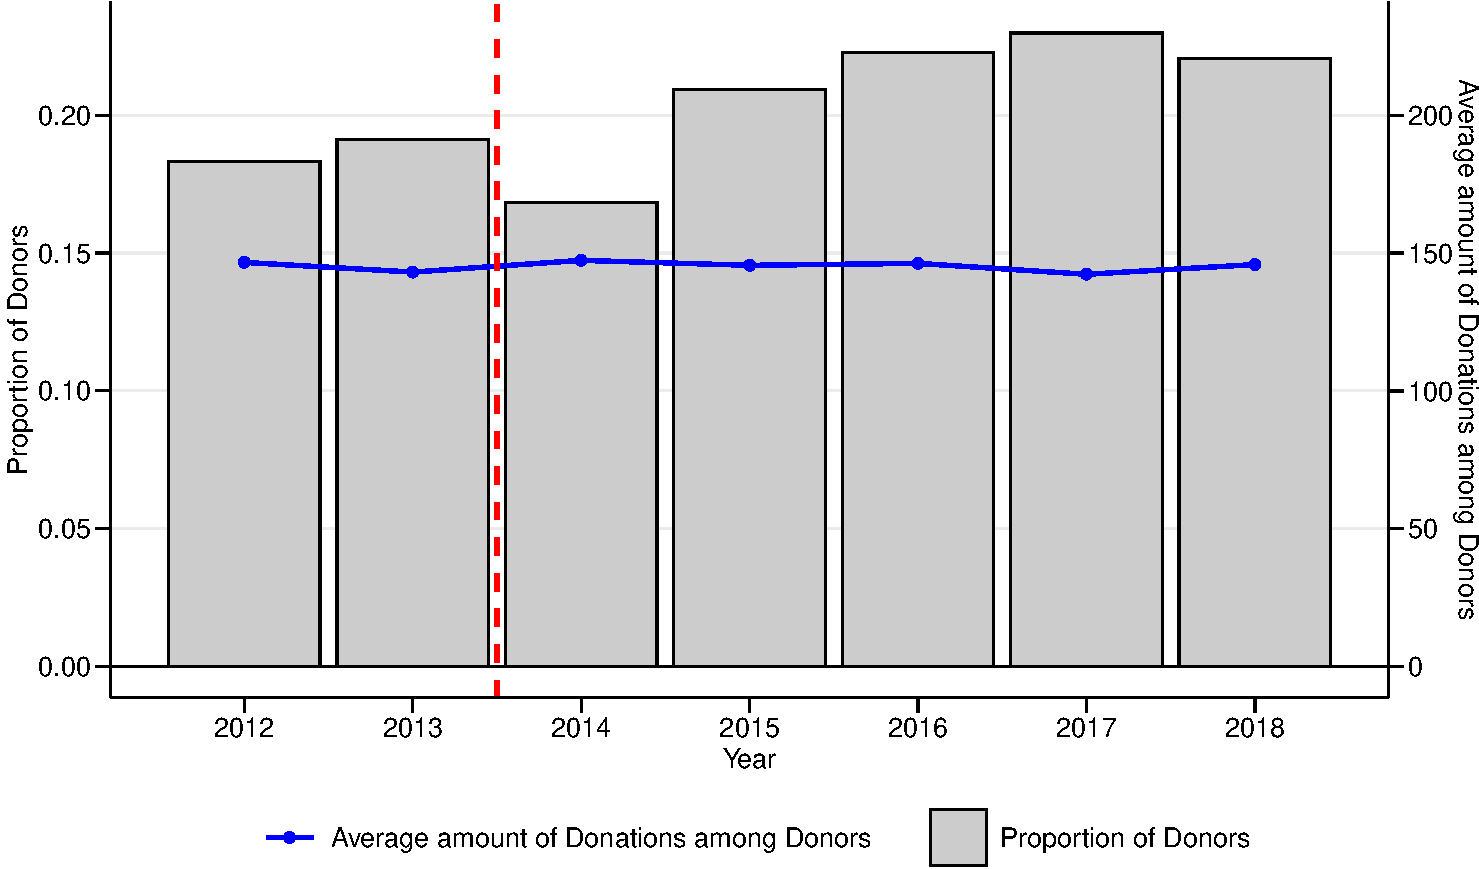
\includegraphics[width=0.9\linewidth]{C:/Users/katoo/Desktop/NASTAB/paper/draft_files/figure-latex/SummaryOutcome-1} 

}

\caption{Proportion of Donors and Average Donations among Donors. Notes: The left and right axises respectively mesure proportion of donors and the average amount donations among donors. Authors made this graph based on NasTaB data.}\label{fig:SummaryOutcome}
\end{figure}

\hypertarget{income-and-giving-price}{%
\subsection{Income and Giving Price}\label{income-and-giving-price}}

NaSTaB asks respondents to answer the annual income last year.
For example, in the 2014 survey, respondents answer the annual income at 2013.
In our sample, the average annual taxable income is 18.76 million KRW.
According to the National Tax Statistical Yearbook published by Korean National Tax Service,
the average annual taxable income is 32.77 million from 2012 to 2018
for employees who submited the tax return.
Since our sample includes subjects with no labor income, such as housewife,
our sample mean of income is lower than average income calculated by the public organizations.
In Figure \ref{fig:showSummaryPriceChange},
the grey bars show the distribution of annual taxable income in 2013.
The income distribution is left-skewed.

Using this variable, we construct the giving price under the tax deduction system (2012 and 2013).
After the tax reform (after 2014), the giving price is 0.85 under the tax credit system,
as we explained in the section \ref{institutional-background}.
In Figure \ref{fig:showSummaryPriceChange},
the blue line shows giving price in 2012 and 2013,
while the red dashed line shows the giving price after 2014.
From this figure,
those whose annual income is less than 1200 in 2013 could receive benefit by the 2014 tax reform
bacause the tax reform decreases the giving price.
On the other hand,
those whose auunal income is greater than 4600 in 2013 had a loss by the 2014 tax reform
since the tax reform increases the giving price.

\begin{figure}[t]

{\centering 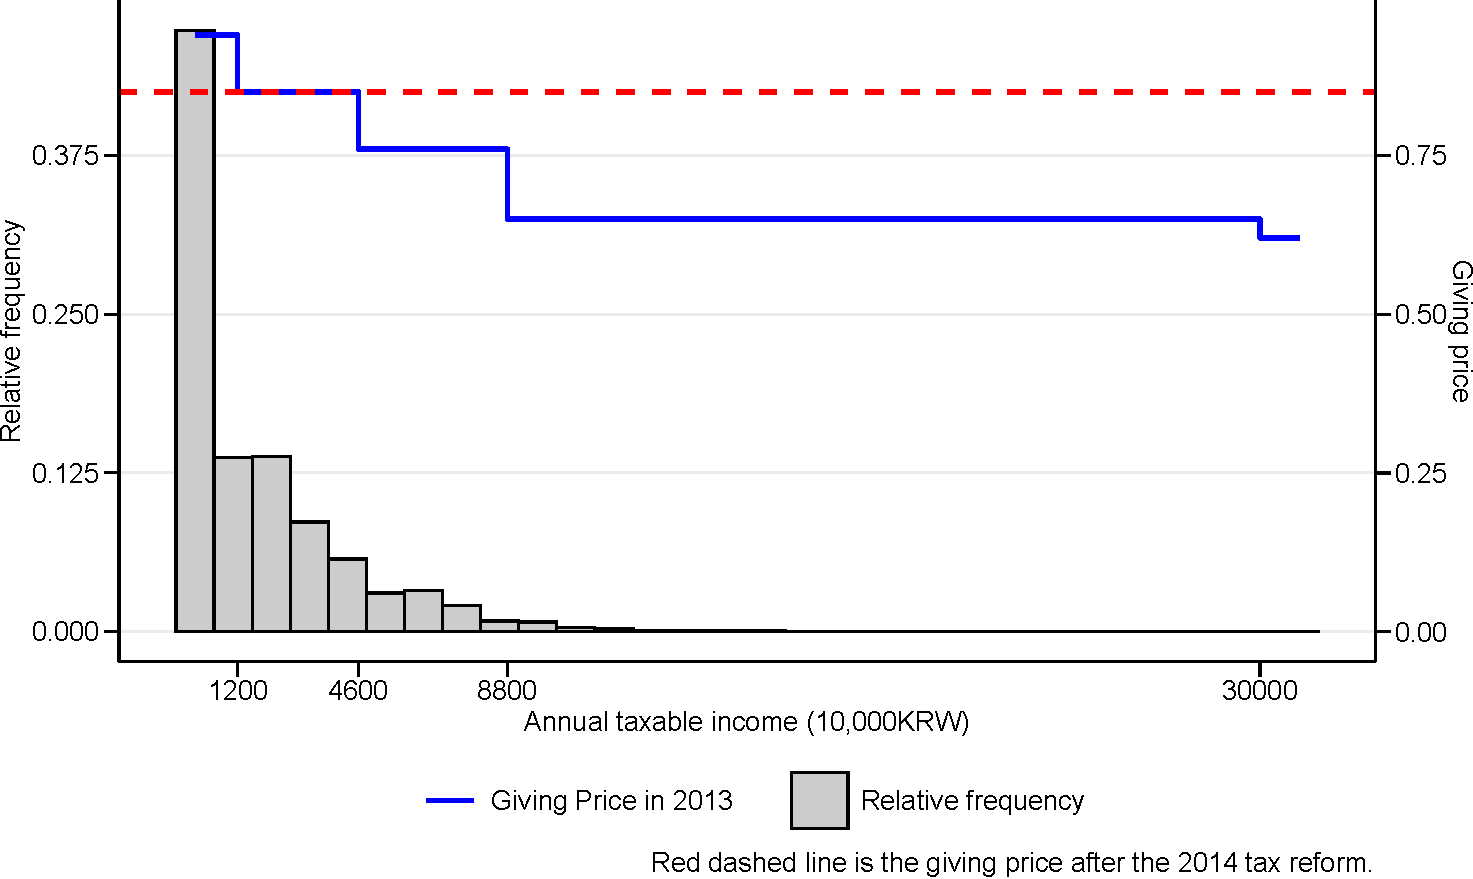
\includegraphics[width=0.9\linewidth]{C:/Users/katoo/Desktop/NASTAB/paper/draft_files/figure-latex/SummaryPriceChange-1} 

}

\caption{Income Distribution and Giving Price in 2013}\label{fig:SummaryPriceChange}
\end{figure}

\clearpage

\hypertarget{references}{%
\section*{References}\label{references}}
\addcontentsline{toc}{section}{References}

\hypertarget{refs}{}
\begin{CSLReferences}{1}{0}
\leavevmode\hypertarget{ref-Almunia2020}{}%
Almunia, M., Guceri, I., Lockwood, B., Scharf, K., 2020. More giving or more givers? The effects of tax incentives on charitable donations in the UK. Journal of Public Economics 183. doi:\href{https://doi.org/10.1016/j.jpubeco.2019.104114}{10.1016/j.jpubeco.2019.104114}

\leavevmode\hypertarget{ref-Anderson2017}{}%
Anderson, J.E., 2017. Trust in government and willingness to pay taxes in transition countries. Comparative Economic Studies 59, 1--22. doi:\href{https://doi.org/10.1057/s41294-016-0017-x}{10.1057/s41294-016-0017-x}

\leavevmode\hypertarget{ref-Auten2002}{}%
Auten, G.E., Sieg, H., Clotfelter, C.T., 2002. Charitable giving, income, and taxes: An analysis of panel data. American Economic Review 92, 371--382.

\leavevmode\hypertarget{ref-Bakija2011}{}%
Bakija, J., Heim, B.T., 2011. How does charitable giving respond to incentives and income? New estimates from panel data. National Tax Journal 64, 615--650. doi:\href{https://doi.org/10.17310/ntj.2011.2S.08}{10.17310/ntj.2011.2S.08}

\leavevmode\hypertarget{ref-Fack2010}{}%
Fack, G., Landais, C., 2010. Are tax incentives for charitable giving efficient? Evidence from france. American Economic Journal - Economic Policy 2, 117--141. doi:\href{https://doi.org/10.1257/pol.2.2.117}{10.1257/pol.2.2.117}

\leavevmode\hypertarget{ref-Frey2007}{}%
Frey, B.S., Torgler, B., 2007. Tax morale and conditional cooperation. Journal of Comparative Economics 35, 136--159. doi:\href{https://doi.org/10.1016/j.jce.2006.10.006}{10.1016/j.jce.2006.10.006}

\leavevmode\hypertarget{ref-Hammar2009}{}%
Hammar, H., Jagers, S.C., Nordblom, K., 2009. Perceived tax evasion and the importance of trust. The Journal of Socio-Economics 38, 238--245. doi:\url{https://doi.org/10.1016/j.socec.2008.07.003}

\leavevmode\hypertarget{ref-Kim2021}{}%
Kim, Y., 2021. Politics, religion, and tax incentives for charitable giving in south korea. Korean Economic Review 37, 141--155. doi:\href{https://doi.org/10.22841/kerdoi.2021.37.1.006}{10.22841/kerdoi.2021.37.1.006}

\leavevmode\hypertarget{ref-Li2011}{}%
Li, S.X., Eckel, C.C., Grossman, P.J., Brown, T.L., 2011. Giving to government: Voluntary taxation in the lab. Journal of Public Economics 95, 1190--1201. doi:\href{https://doi.org/10.1016/j.jpubeco.2011.03.005}{10.1016/j.jpubeco.2011.03.005}

\leavevmode\hypertarget{ref-Randolph1995}{}%
Randolph, W.C., 1995. Dynamic income, progressive taxes, and the timing of charitable contributions. Journal of Political Economy 103, 709--738. doi:\href{https://doi.org/10.1086/262000}{10.1086/262000}

\leavevmode\hypertarget{ref-Saez2004}{}%
Saez, E., 2004. The optimal treatment of tax expenditures. Journal of Public Economics 88, 2657--2684. doi:\href{https://doi.org/10.1016/j.jpubeco.2003.09.004}{10.1016/j.jpubeco.2003.09.004}

\leavevmode\hypertarget{ref-Sheremeta2020}{}%
Sheremeta, R.M., Uler, N., 2020. The impact of taxes and wasteful government spending on giving. Experimental Economics. doi:\href{https://doi.org/10.1007/s10683-020-09673-9}{10.1007/s10683-020-09673-9}

\end{CSLReferences}

\end{document}
